A transformada discreta de Fourier (DFT), bem como sua versão otimizada --- a transformada rápida de Fourier
(FFT) --- possui diversas aplicações, entre elas o processamento e a filtragem de sinais temporais discretizados.

Vamos explorar essa técnica para atenuar eventuais ruídos de medição presentes em um sinal de tensão amostrado,
realçando suas componentes harmônicas relevantes.

\subsection*{Etapa 1}
Desenvolva um script que sintetize a evolução temporal da tensão em uma fase da rede de baixa tensão.
A discretização do sinal deve conter 1024\footnote{Para que essa técnica seja empregada de forma eficiente,
    é necessário que o número de amostras do sinal corresponda a uma potência de dois.} amostras uniformemente no
intervalo de tempo entre 0 e 50ms.
A forma de onda resultante deve incluir uma componente fundamental com valor eficaz de 220V e frequência de 60Hz,
além de uma componente harmônica de $5^a$ ordem com valor eficaz de 40V e fase de $128.4^\circ$.
Adicione também um ruído aleatório com amplitude de 300V e média nula (consulte a \inlcode{np.random.rand}).



\subsection*{Etapa 2}
Utilize as funções do módulo \inlcode{numpy.fft}
para calcular a transformada de Fourier do sinal gerado na etapa anterior, determinando a amplitude de cada componente
de frequência presente em seu espectro.

Em seguida, filtre o espectro resultante, zerando as componentes cuja magnitude seja inferior a $10 \cdot 1024$.

Aplique a transformada inversa de Fourier (\inlcode{ifft}) para reconstruir o sinal de tensão já filtrado.

Por fim, gere um gráfico comparativo  que sobreponha o sinal filtrado ao sinal original, de forma a destacar
visualmente os efeitos do processo de filtragem, conforme exemplificado na \figr{fig:fft}.
\begin{figure}[htbp]
    \centering
    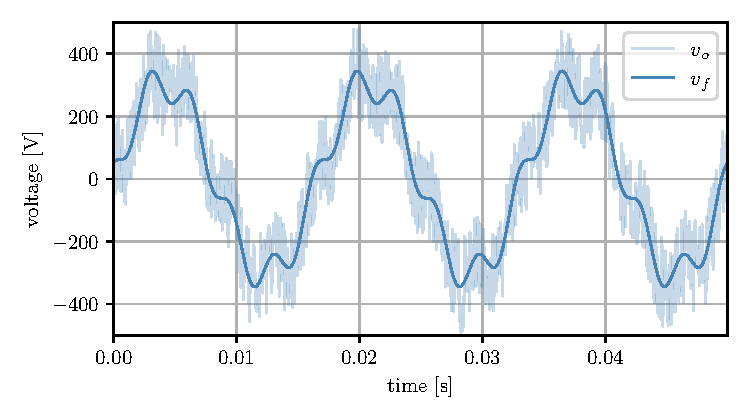
\includegraphics[scale=1.0]{figs/fft}
    \caption{Resultado esperado.}
    \label{fig:fft}
\end{figure}
